\documentclass[11pt]{article}
\usepackage{geometry}                % See geometry.pdf to learn the layout options. There are lots.
\geometry{letterpaper}                   % ... or a4paper or a5paper or ... 
%\geometry{landscape}                % Activate for for rotated page geometry
%\usepackage[parfill]{parskip}    % Activate to begin paragraphs with an empty line rather than an indent
\usepackage{graphicx}
\usepackage{tikz}
\usepackage{amssymb}
\usepackage{pgfplots}
\usepackage{amsmath}
\usepackage{caption}
\usepackage{subcaption}
\pgfplotsset{compat=newest}
\usetikzlibrary{calc,decorations,decorations.pathreplacing}
\usepackage{epstopdf}
\DeclareGraphicsRule{.tif}{png}{.png}{`convert #1 `dirname #1`/`basename #1 .tif`.png}

\title{Numerical Simulation}
\date{}                                           % Activate to display a given date or no date

\begin{document}
\maketitle
\section{Background}
A large part of this thesis concerns the motion of many bodies in the presence of a Kerr black hole.  I give each body a Newtonian gravitational potential and look at how that affects their trajectories.  I now present the ``n-body problem" and explain briefly why it is difficult and what techniques I employ to solve it computationally.
\subsection{The N-Body Problem}\label{sec:nbody-intro}
Presented with two bodies which interact purely gravitationally \--- planets, stars, grains of dust \--- I can write an equation which will give me the position of each body at any point in time.  This problem has been solved since the 18\textsuperscript{th} century and follows pretty naturally from Newton's observation that the force of gravity between two bodies falls off as the inverse square of the distance between them.  We can write this mathematically as
\begin{equation*}
\mathbf{F}_1 = \mathbf{F}_{12} = \frac{1}{r_{12}^2}G m_1 m_2\mathbf{\hat{r}}_{12},
\end{equation*}

 for two bodies, of masses $m_1$ and $m_2$, respectively.  $G$ is the gravitational constant, and $r_{12}$ is the distance between the body 1 and body 2.   $\mathbf{\hat{r}_{12}}$ is a vector that points from one body to the other (Fig. \ref{fig:2body}).  Here, ``$\mathbf{F_1}$" is the force on body 1, and ``$\mathbf{F}_{12}$" is the force on body 1 \emph{due to} body 2, so it is read ``F-one-two" and not ``F-twelve" (and likewise for $r_{12}$).  In this case, $\mathbf{F}_1$ and $\mathbf{F}_{12}$ are equal, but that is not always true as we will see in a second. 


As I said, the problem for the gravitational interaction between two bodies is totally solved.  However, if I introduce a third body (Fig. \ref{fig:3body}), the story is made murky:  Now each of the planets or stars or whatever is being pulled simultaneously by \emph{two} other bodies.  The force on any one body at a given instant is described by the sum of the forces due to the other two bodies.  For instance, the force on the first body would be given by
\begin{align*}
\mathbf{F}_1 &= \mathbf{F}_{12}+\mathbf{F}_{13}\\
&= \frac{1}{r_{12}^2}G m_1 m_2 \mathbf{\hat{r}}_{12} +  \frac{1}{r_{13}^2}G m_1 m_3 \mathbf{\hat{r}}_{13}
\end{align*}

This will move body 1 in some direction, but bodies 2 and 3 are \emph{also} experiencing gravitational pulls and so they too are constantly moving around. So the total force on any given body is constantly changing in direction and magnitude.

\begin{figure}[ht]
\centering
\begin{subfigure}[t]{.5\textwidth}
  \centering
\includegraphics[scale=0.35]{/Users/alexdeich/Desktop/2body.png}
  \captionof{figure}{}
  \label{fig:2body}
\end{subfigure}%
\hfill
\begin{subfigure}[t]{.5\textwidth}
  \centering
  \includegraphics[scale=0.35]{/Users/alexdeich/Desktop/3body.png}
  \captionof{figure}{}
  \label{fig:3body}
\end{subfigure}
\caption{On the left, two bodies are being influenced by each other's gravitational pull.  The force that $m_2$ experiences is equal in magnitude to the force that $m_1$ experiences, but in the opposite direction.  With 3 or more bodies (depicted on the right), ``equal and opposite" has no meaning\--- each body feels the sum of the pull from every other body.}
\end{figure}

It turns out, unlike for the 2-body case, it is impossible to write an equation which will totally describe the positions of all three bodies at any point in time.  In fact, this is true for \emph{any} number of gravitationally interacting bodies greater than 2.  The problem of determining these positions after some amount of time is dubbed the \emph{n-body problem}.

\subsection{Solution: Time Stepping}
In order to model systems of many gravitationally interacting bodies, then, we need another method, and so we come to \emph{time stepping}.  Time stepping comes from the observation that if we know the force on a given particle, we know exactly how that particle will move, \emph{assuming the force is constant}.  This follows from the equations of kinematics.  For instance, if there is a particle with mass $m$ at position $\mathbf{x}_0$ with velocity $\mathbf{v}_0$, we know that in some time interval $\Delta t$, its new position $\mathbf{x}_1$ will be given by
\begin{equation*}
\mathbf{x}_1=\mathbf{x}_0 + \mathbf{v}_0 \Delta t.
\end{equation*}
But if that particle is experiencing some force, $\mathbf{F}$, then its velocity will also change: after time $\Delta t$, it will be accelerated to a new velocity, $\mathbf{v}_1$.  We need another equation to describe this.  The acceleration on the particle is just the force divided by its mass, $\mathbf{a} = \mathbf{F}/m$, and so the particle's position and velocity change in time $\Delta t$ according to

\begin{align*}
\mathbf{x}_1&=\mathbf{x}_0 + \mathbf{v}_0 \Delta t.\\
\mathbf{v}_1&=\mathbf{v}_0 + \mathbf{a} \Delta t.
\end{align*}

Thus we can totally describe the motion of a particle under a force \emph{assuming the force is constant}.  But how does this help us?  Section \ref{sec:nbody-intro} was all about how the forces in the n-body problem are extremely \emph{un}constant.  

If we're being exact, that's true.  In some time $\Delta t$, the bodies will move around, and the distances between each body will change, and so the force will change as well.  But if we make $\Delta t$ quite small, then to very good approximation, the force will stay constant \emph{in that time interval}.  Then we can move the bodies around as if the force on each is constant in that interval, then at the end of that interval, reevaluate their positions, calculate new forces, and move them again for the same amount of time, and repeat.   The smaller we make $\Delta t$, the more accurate the approximation is.

Each $\Delta t$ is usually called a \emph{time step}, and this describes the method of time stepping.  The whole process described above is presented as a flowchart in Fig. \ref{fig:nbody_flow}.  This approximation technique is how we can probe the behavior of n-body systems.  Of course, this can extremely computationally intensive.  In a system with 10,000 bodies, calculating the force on any given body in a single time step is a total nightmare for a human.  It is only because of computers that time stepping is possible, and even then, there are many optimization methods we must use to make the problem tractable.

Finally, because the process above discretely solves the integral,

\begin{equation}
x = \int_{t_0}^{t_f} v(t)dt,
\end{equation}

it is called \emph{numerical integration}.

\begin{figure}[ht]
\begin{center}
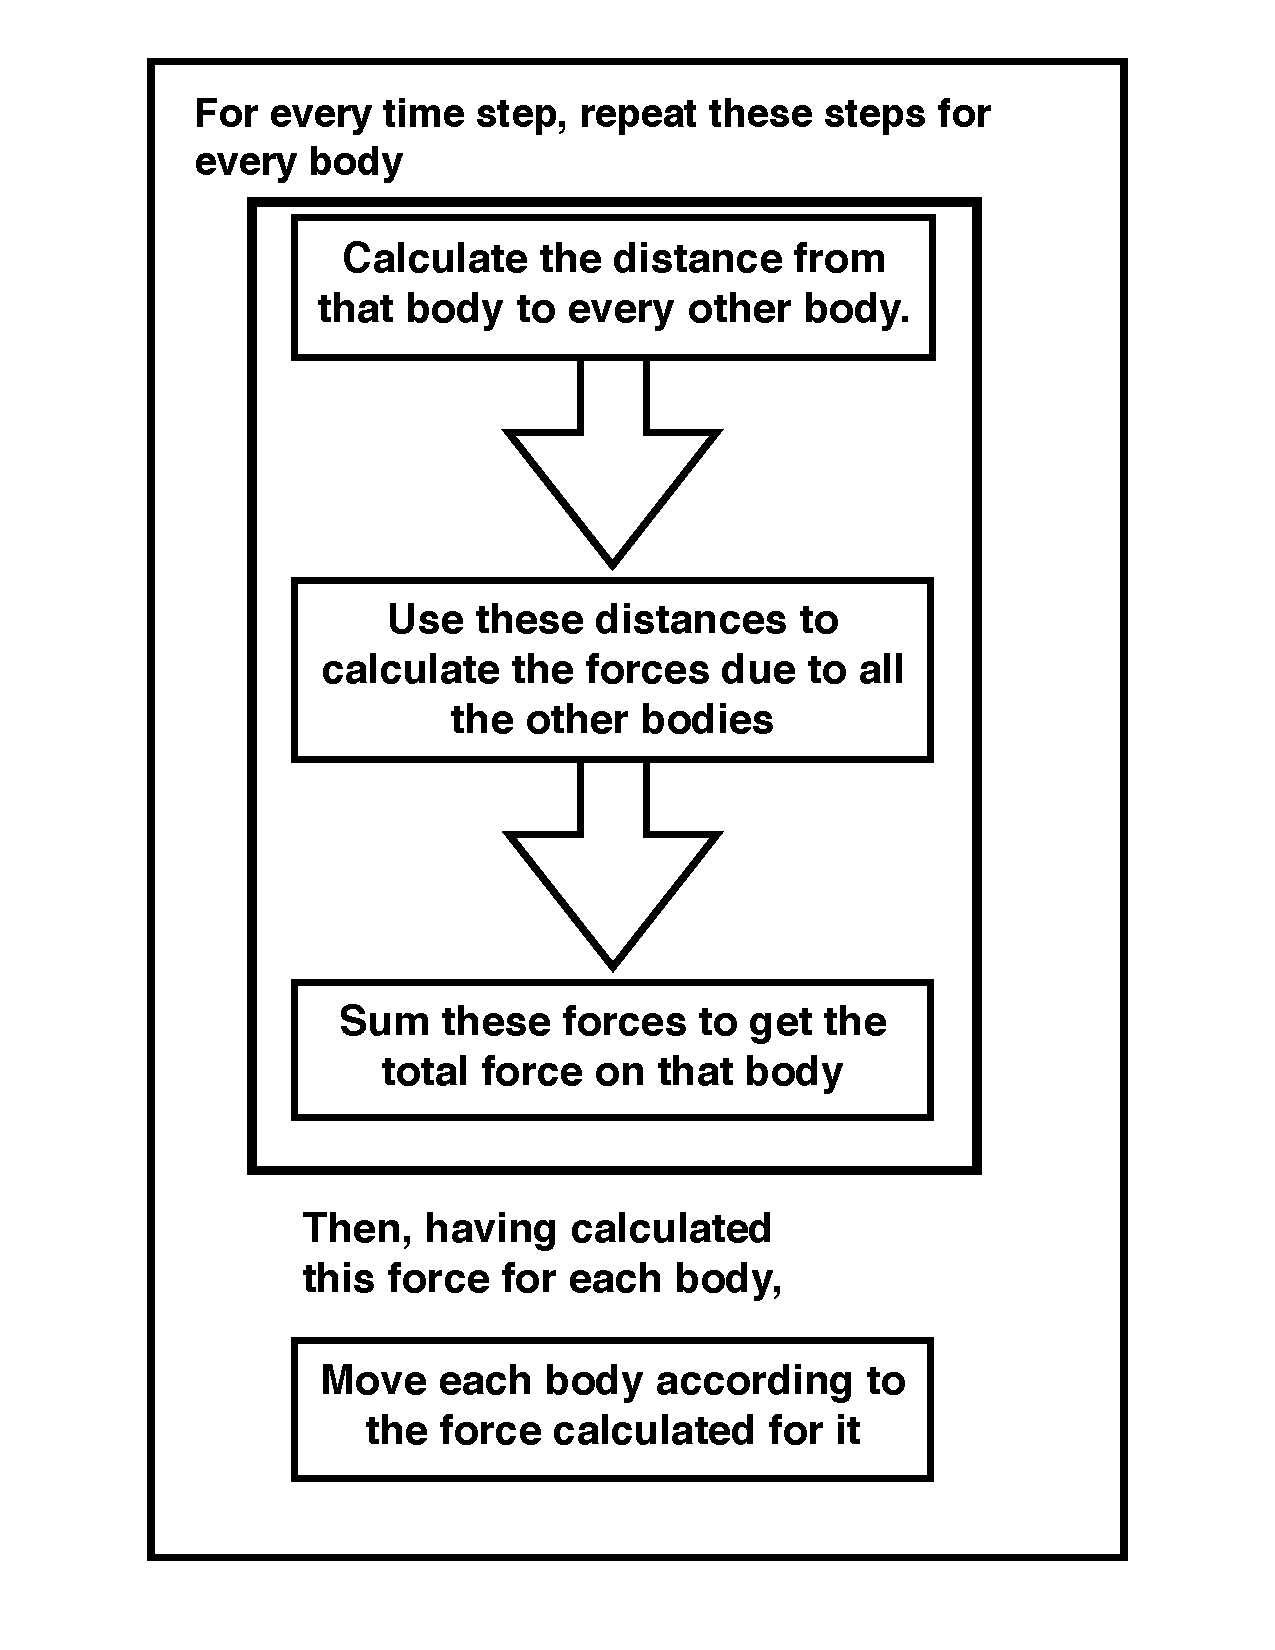
\includegraphics[scale=0.40]{/Users/alexdeich/Dropbox/thesis/latex/nbody_latex/nbody_alg.pdf}
\caption{The algorithm for time-stepping an n-body system.}
\label{fig:nbody_flow}
\end{center}
\end{figure}
\newpage
\section{Numerical Integrations used in this Thesis}

This thesis uses a fourth-order Runge-Kutta method to solve for the trajectories of particles whose equations of motion are given by the Kerr line element.  What follows is a description of the method and its specific implementation in the code used for analysis.

\subsection{Fourth-Order Runge-Kutta}
The fourth-order Runge-Kutta (RK4) method is a numerical integration method frequently used in temporal discretization problems.

Let an initial value problem be specified like so:
\begin{align*}
\mathbf{\dot{x}} = \mathbf{f}(t,\mathbf{x})\\
\mathbf{x}(t_0) = \mathbf{y_0}
\end{align*}

Where $\mathbf{x}$ represents the (vector) function of time (position, in our case) we want to integrate.  In this example, the time-derivative, $\mathbf{\dot{x}}$ be a function of $t$ and $\mathbf{x}$, but it doesn't have to be.  The value of the function $\mathbf{x}$ at $t_0$ is $\mathbf{x_0}$, and both this initial value and the initial time $t_0$ are given.

RK4, then works like this:\\
For a given step size $dt$, the $n^{th}$ steps in position and time are given by

\begin{align}\label{eq:rk4-def}
&\mathbf{x}_{n+1} = \mathbf{x}_n+\frac{dt}{3}\left(\frac{\mathbf{k}_1}{2}+\mathbf{k}_2+\mathbf{k}_3+\frac{\mathbf{k}_4}{2}\right)\\
&t_{n+1} = t_n + dt
\end{align}

The $\mathbf{k}_{1\dots4}$ are given by:

\begin{align}
&\mathbf{k}_1 = f(t_n,\mathbf{x}_n)\\
&\mathbf{k}_2 = f(t_n+\frac{dt}{2},\mathbf{x}_n+\frac{dt}{2}\mathbf{k}_1)\\
&\mathbf{k}_3 = f(t_n+\frac{dt}{2},\mathbf{x}_n+\frac{dt}{2}\mathbf{k}_2)\\
&\mathbf{k}_4 =  f(t_n+dt,\mathbf{x}_n+dt\mathbf{k}_3)
\end{align}

So the $\mathbf{k}_{1\dots4}$ can be thought of as interstitial time-steps, each using a different method, which are all then combined in some kind of fancy average in (\ref{eq:rk4-def}).  For the example, it is clear that $\mathbf{k}_1$ is just a straight-forward Euler's method, as it's using information about the slope at the beginning of the interval to update the vector.  Likewise, $\mathbf{k}_2$ and $\mathbf{k}_3$ are midpoint methods.  To understand exactly why the various methods are combined like they are in (\ref{eq:rk4-def}) requires a full derivation, which can be found in [1].  


\subsection{The Equations of Motion}
As I derived earlier, equations of motion generated by solving for geodesics in Kerr spacetime are unwieldy and totally unhelpful in forming any sort of intuition.  Therefore, for the current discussion I adopt the subscript $K$ when referring to a coordinate's equation of motion due to Kerr.

When confined to the disk, I consider motion in $r$ and $\phi$.  The derivative vector I update with is then 
\begin{align}
\left(
\begin{array}{c}
\dot{r} \\
\ddot{r}_K+\ddot{r}_{ext.} \\
\dot{\phi} \\
\ddot{\phi}_K+\ddot{\phi}_{ext.} \\
\end{array}
\right)
\end{align}
Where the $\ddot{r}_{ext.}$ and $\ddot{\phi}_{ext.}$ are some accelerations given by various external forces, depending on what I'm testing in that given integration.

\subsection{External Forces}
My code has methods for calculating three different types of particle-particle interactions, which can in turn be combined with each other.
\subsubsection{Classical N-Body}
This returns the acceleration on a particle due to a Newtonian $r^{-2}$ potential of all other particles.  "Classical" refers to the fact that it uses a Pythagorean sense of length to calculate $r$, which is not relevant in a general relativistic context.

\subsubsection{Classical Elastic Collision}
This edits the state vector for any two colliding particles, and gives them new velocities such that momentum and energy are conserved according to a classical 2-dimensional elastic collision.

\subsubsection{Classical Inelastic Collision}
This is similar to above, but removes the two particles from the state vector and adds a third with the aggregate mass and conserved momentum and energy.

\end{document}  















